\documentclass[10pt, onecolumn, compsoc, conference]{IEEEtran}

\usepackage{etoolbox}
\usepackage{scrextend}
\usepackage{graphicx}
\usepackage[style=numeric,sorting=none]{biblatex}

% remove \centering from \section
\patchcmd{\section}{\centering}{}{}{}

\addbibresource{references.bib}


\begin{document}
\title{An Analysis of Risk in \\Open-Source Project Dependenciess}

\author{\IEEEauthorblockN{Róisín Ní Bhriain}
\IEEEauthorblockA{Student Number: 23269640}
\and
\IEEEauthorblockN{Sneha Dechamma Mallengada Suresh}
    \IEEEauthorblockA{Student Number: 23262168}}

\maketitle

\begin{description}
    \item[]
    \begin{center}
        \item[\textbf{Technical Manual - 23-07-2024}] 
        \end{center}
    \item[]
\end{description}



\begin{abstract}
\begin{addmargin}[4.2em]{4.2em}
This paper explores the methods used in the prediction of risk when using open-source software. There are a number of methods used and the aim is to combine these to give a more comprehensive view of the risks in using a particular open-source project. We examine the literature to decide on an appropriate prediction algorithm for each section. We aim to develop a tool to investigate the risks in Maven dependency trees. We provide a graph of the final results which can be used to aid in finding where the risk lies in the dependency trees. 
\end{addmargin}
\end{abstract}


\section{Introduction}
This paper explores the prediction of risks in Maven dependency trees through examining both GitHub project activity and NVD vulnerability CVE data. ARIMA prediction is used for both sets of data based on user configuration data and returns a coloured graph based on the analysed risk. 

\section{Related Work}
In this section, we review relevant work in the prediction of risk in open-source software. We examine the machine learning models used as well as the different objects of analysis used in the predictions.  

\subsection{Project Metadata Analysis}


\subsection{Vulnerability CVE Data Analysis}
\section{Case Studies}
In this section we will identify a number of case studies where a tool like this would have been valuable to see whether a project depended on a risky project. 

\subsection{Log4j}
In November 2021 a vulnerability was discovered in the popular open-source logging library Apache Log4j. This software is widely used in web portals. The vulnerability in this package means that hackers can run malicious code remotely on a victim's machine \cite{h_gupta_identification_2022}. The main aim of the log4j vulnerability is to obtain Lightweight Directory Access Protocol information and this will serve as a gateway to full control of the machine. The attack works with several steps: information gathering, weaponisation, delivery, exploitation and installation \cite{f_maulana_unmasking_2023}. Once these vulnerabilities were reported a user could use the project to discover that some of their dependencies have vulnerabilities and are thus classed as risky. 


\section{Methodology}
This paper explores the creation of a tool to predict risk in dependency trees. We aim to combine two of the objects of analysis to give a more well rounded analysis vs focusing on one. In this section we initially describe the data we used and then the prediction methods as well as the calculations of risk that we used. 

\subsection{Finding Dependencies Algorithm}

\subsection{Project Meta-Data Prediction}

\subsection{Vulnerability Database Prediction}

\subsection{Risk Calculations}
In terms of calculating risk we implemented some configurations options for a user to decide how many commits, days-to-close issues, and vulnerabilities per month are acceptable. 

\[ projectActivityScore = ( x / numDaysToFixIssues ) * 10\]

\[ projectActivityScore = ( numCommits / x ) * 10\]

\[vulnerabilityScore = ( x / vulsCountPerMonth ) * 10\]

\[overallScore = ( projectActivityScore + vulnerabilityScore) / 2\]


These are the calculations we used for the risk scores for each of the sections. There is the option to decide project activity based on issues fix time, commits per month or both. The user supplies the configuration options of \textit{numDaysToFixIssues}, \textit{numCommits}, and \textit{vulCountsPerMonth}. That way the acceptable levels of risk are set. The idea is that they are then assigned a risk score: where not enough is < 0, 0-2.5 is low risk, 2.5-5 is medium risk, 5-7.5 is high risk and > 7.5 is severe risk. 

\begin{figure}
    \centering
    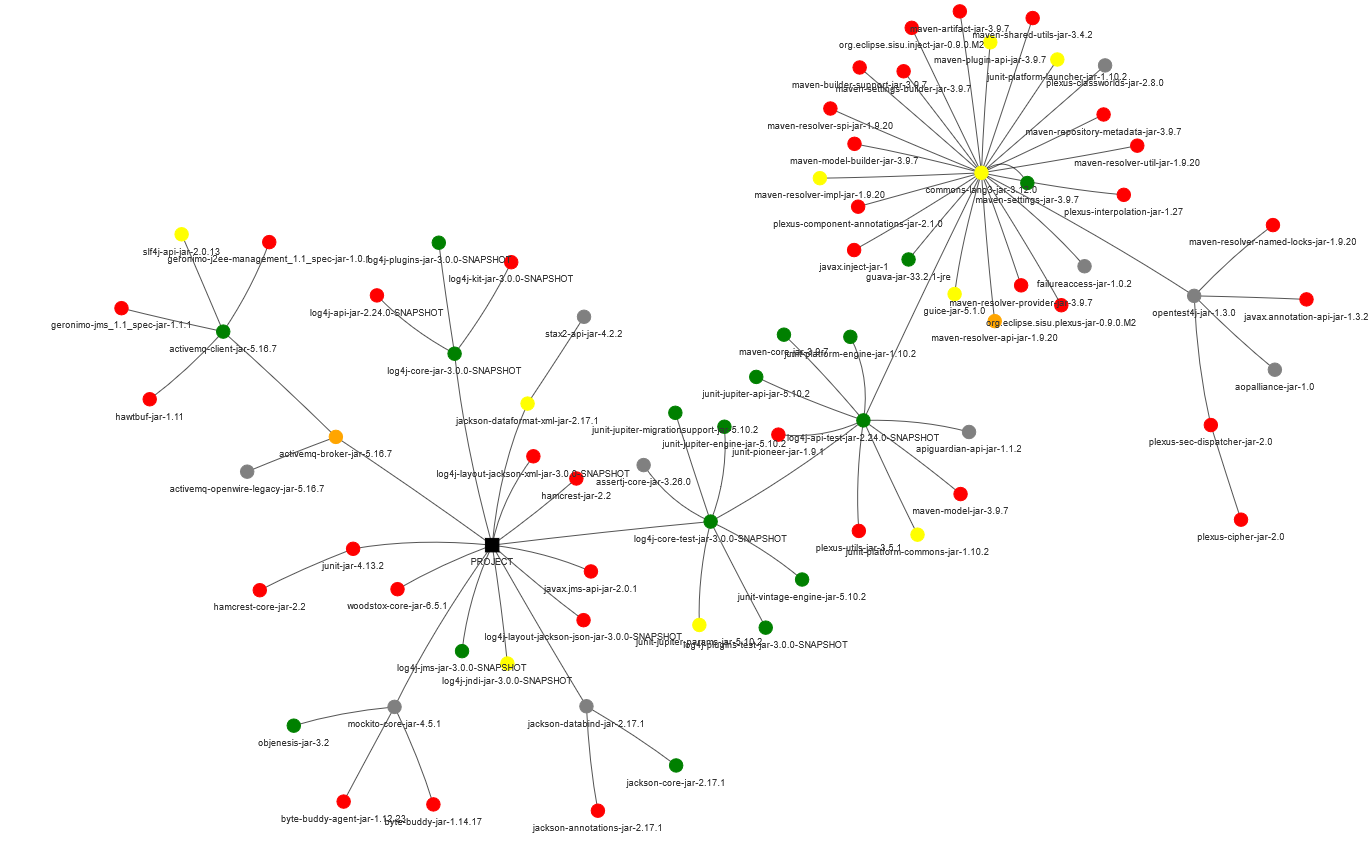
\includegraphics[width=01\linewidth]{image.png}
    \caption{Dependency Tree Results With Risk Levels Colour Coded} 
\end{figure}

Figure 1 shows a final dependency tree with colour coded risk evaluations of each of the dependencies.This figure was based on a user configuration of two vulnerabilities being acceptable and 70 being the minimum number of commits per month as acceptable. 


\section{Results \& Evaluation}
To evaluate the algorithm we used a number of different maven projects with different dependencies. We made sure to use some projects that were discussed as above in the case studies section. We used a Log4j maven sample project. 

We found that the project activity predictions generally performed a lot better than the vulnerability CVE data - presumably due to a lack of data in the NVD databases (which can in some cases mean no vulnerabilities - a good thing). A lot of the dependencies were also grouped in the same projects on GitHub which meant that there was only the need to calculate the prediction for these once. An issue we ran into was that there was no way of automatically using an API to find the GitHub projects of the dependencies - this meant we had to manually go through each of the dependency trees and find the project URLs on GitHub which does not bode well for scaling the project up for larger Maven projects. 

For the evaluation of the predictions in this project we used the commonly used metrics: Mean absolute percentage error (MAPE), mean absolute error (MAE), and root mean squared error (RMSE). 

\section{Conclusions \& Further Work}
For the purpose of this paper we focused on examining Maven dependency trees which is primarily used for Java projects. Further work could be done to examine other package manager dependency trees such as \textit{PyPI} for Python, \textit{NPM} for JavaScript, and \textit{Conan} for C. 

\printbibliography

\appendices
\section{Graphs}
This section contains other important graphs that we did not include in the main body of the project.

\ifCLASSOPTIONcaptionsoff
  \newpage
\fi

\end{document}